
%%%%%%%%%%%%%%%%%%%%%%%%%%%%%%%%%%%%%%%%%%%%%%%%%%%%%%%%%%%%%%%%%%%%%
%% This is a (brief) model paper using the achemso class
%% The document class accepts keyval options, which should include
%% the target journal and optionally the manuscript type.
%%%%%%%%%%%%%%%%%%%%%%%%%%%%%%%%%%%%%%%%%%%%%%%%%%%%%%%%%%%%%%%%%%%%%
\documentclass[journal=jacsat,biochem,manuscript=article]{achemso}

%%%%%%%%%%%%%%%%%%%%%%%%%%%%%%%%%%%%%%%%%%%%%%%%%%%%%%%%%%%%%%%%%%%%%
%% Place any additional packages needed here.  Only include packages
%% which are essential, to avoid problems later. Do NOT use any
%% packages which require e-TeX (for example etoolbox): the e-TeX
%% extensions are not currently available on the ACS conversion
%% servers.
%%%%%%%%%%%%%%%%%%%%%%%%%%%%%%%%%%%%%%%%%%%%%%%%%%%%%%%%%%%%%%%%%%%%%
%%\usepackage[version=3]{mhchem} % Formula subscripts using \ce{}
\usepackage{mciteplus}
\usepackage[T1]{fontenc}       % Use modern font encodings
\usepackage{hyperref}

\usepackage{xcolor}
\usepackage{ulem}

%%%%%%%%%%%%%%%%%%%%%%%%%%%%%%%%%%%%%%%%%%%%%%%%%%%%%%%%%%%%%%%%%%%%%
%% If issues arise when submitting your manuscript, you may want to
%% un-comment the next line.  This provides information on the
%% version of every file you have used.
%%%%%%%%%%%%%%%%%%%%%%%%%%%%%%%%%%%%%%%%%%%%%%%%%%%%%%%%%%%%%%%%%%%%%
%%\listfiles

%%%%%%%%%%%%%%%%%%%%%%%%%%%%%%%%%%%%%%%%%%%%%%%%%%%%%%%%%%%%%%%%%%%%%  
%% Place any additional macros here.  Please use \newcommand* where
%% possible, and avoid layout-changing macros (which are not used
%% when typesetting).
%%%%%%%%%%%%%%%%%%%%%%%%%%%%%%%%%%%%%%%%%%%%%%%%%%%%%%%%%%%%%%%%%%%%%
\newcommand*\mycommand[1]{\texttt{\emph{#1}}}
\newcommand*\fref[1]{Figure~\ref{fig:#1}}
\newcommand*\tref[1]{Table~\ref{table:#1}}
\newcommand*\sref[1]{Section~\ref{sec:#1}}
\newcommand*\eg{e.g.,~}
\newcommand*\ie{i.e.,~}
\newcommand*\vs{vs.~}
\newcommand*\viz{viz.~}
%\newcommand*\citeauthoryear[1]{{\citeauthor{#1}~(\citeyear{#1})}}

%%%%%%%%%%%%%%%%%%%%%%%%%%%%%%%%%%%%%%%%%%%%%%%%%%%%%%%%%%%%%%%%%%%%%
%% Meta-data block
%% ---------------
%% Each author should be given as a separate \author command.
%%
%% Corresponding authors should have an e-mail given after the author
%% name as an \email command. Phone and fax numbers can be given
%% using \phone and \fax, respectively; this information is optional.
%%
%% The affiliation of authors is given after the authors; each
%% \affiliation command applies to all preceding authors not already
%% assigned an affiliation.
%%
%% The affiliation takes an option argument for the short name.  This
%% will typically be something like "University of Somewhere".
%%
%% The \altaffiliation macro should be used for new address, etc.
%% On the other hand, \alsoaffiliation is used on a per author basis
%% when authors are associated with multiple institutions.
%%%%%%%%%%%%%%%%%%%%%%%%%%%%%%%%%%%%%%%%%%%%%%%%%%%%%%%%%%%%%%%%%%%%%
\author{Deepak Bandyopadhyay}
\email{debug22@gmail.com}
\altaffiliation{Current address: Janssen Pharmaceutical Companies of Johnson and Johnson, McKean and Welsh Roads, Spring House, PA 19477}
\author{Constantine Kreatsoulas}
\author{Pat G. Brady}
\author{Joseph Boyer}
\author{Zangdong He}
\author{Genaro Scavello Jr.}
\affiliation[GSK]{GlaxoSmithKline, 1250 S. Collegeville Rd, Collegeville, PA 19426}
\author{Tyler Peryea}
\author{Ajit Jadhav}
\author{Dac-Trung Nguyen}
\email{nguyenda@mail.nih.gov}
\author{Rajarshi Guha}
\email{rajarshi\_guha@vrtx.com}
%\phone{+123 (0)123 4445556}
%\fax{+123 (0)123 4445557}
\affiliation[NCATS]{National Center for Advancing Translational
  Science, 9800 Medical Center Drive, Rockville, MD 20850}
\altaffiliation{Current address: Vertex Pharmaceuticals, 50 Northern Avenue, Boston MA 02210}

%%%%%%%%%%%%%%%%%%%%%%%%%%%%%%%%%%%%%%%%%%%%%%%%%%%%%%%%%%%%%%%%%%%%%
%% The document title should be given as usual. Some journals require
%% a running title from the author: this should be supplied as an
%% optional argument to \title.
%%%%%%%%%%%%%%%%%%%%%%%%%%%%%%%%%%%%%%%%%%%%%%%%%%%%%%%%%%%%%%%%%%%%%
\title[Scaffold Analytics] {Scaffold-Based Analytics: Enabling Hit-to-Lead
  Decisions by Visualizing Chemical Series Linked Across Large Datasets}  

%%%%%%%%%%%%%%%%%%%%%%%%%%%%%%%%%%%%%%%%%%%%%%%%%%%%%%%%%%%%%%%%%%%%%
%% Some journals require a list of abbreviations or keywords to be
%% supplied. These should be set up here, and will be printed after
%% the title and author information, if needed.
%%%%%%%%%%%%%%%%%%%%%%%%%%%%%%%%%%%%%%%%%%%%%%%%%%%%%%%%%%%%%%%%%%%%%
%\abbreviations{IR,NMR,UV}
%\keywords{American Chemical Society, \LaTeX}

%%%%%%%%%%%%%%%%%%%%%%%%%%%%%%%%%%%%%%%%%%%%%%%%%%%%%%%%%%%%%%%%%%%%%
%% The manuscript does not need to include \maketitle, which is
%% executed automatically.
%%%%%%%%%%%%%%%%%%%%%%%%%%%%%%%%%%%%%%%%%%%%%%%%%%%%%%%%%%%%%%%%%%%%%
\begin{document}

%%%%%%%%%%%%%%%%%%%%%%%%%%%%%%%%%%%%%%%%%%%%%%%%%%%%%%%%%%%%%%%%%%%%%
%% The "tocentry" environment can be used to create an entry for the
%% graphical table of contents. It is given here as some journals
%% require that it is printed as part of the abstract page. It will
%% be automatically moved as appropriate.
%%%%%%%%%%%%%%%%%%%%%%%%%%%%%%%%%%%%%%%%%%%%%%%%%%%%%%%%%%%%%%%%%%%%%
%\begin{tocentry}

%Some journals require a graphical entry for the Table of Contents.
%This should be laid out ``print ready'' so that the sizing of the
%text is correct.

%Inside the \texttt{tocentry} environment, the font used is Helvetica
%8\,pt, as required by \emph{Journal of the American Chemical
%Society}.

%The surrounding frame is 9\,cm by 3.5\,cm, which is the maximum
%permitted for  \emph{Journal of the American Chemical Society}
%graphical table of content entries. The box will not resize if the
%content is too big: instead it will overflow the edge of the box.

%This box and the associated title will always be printed on a
%separate page at the end of the document.

%\end{tocentry}

%%%%%%%%%%%%%%%%%%%%%%%%%%%%%%%%%%%%%%%%%%%%%%%%%%%%%%%%%%%%%%%%%%%%%
%% The abstract environment will automatically gobble the contents
%% if an abstract is not used by the target journal.
%%%%%%%%%%%%%%%%%%%%%%%%%%%%%%%%%%%%%%%%%%%%%%%%%%%%%%%%%%%%%%%%%%%%%
\begin{abstract}
  We present a method for visualizing and navigating large screening
  datasets, taking into account their activities and properties. Our
  approach is to annotate the data with all possible scaffolds
  contained within each molecule.  We have developed a Spotfire
  visualization, coupled to a fuzzy clustering approach based on the
  scaffold decomposition of the screening deck, that is used to drive
  the hit triage process. Progression decisions can be made using
  aggregate scaffold parameters and data from multiple datasets merged
  at the scaffold level.  This visualization reveals overlaps
  that help prioritize hits, highlight tractable series and posit ways
  to combine aspects of multiple hits.  The SAR of a large and complex
  hit is automatically mapped onto all constituent scaffolds making it
  possible to navigate, via any shared scaffold, to all related hits.
  This scaffold ``walking'' helps address bias toward a handful of
  potent and ligand-efficient molecules at the expense of coverage of
  chemical space.  We consider two scaffold generation methods and
  explored their similarities and differences both qualitatively and
  quantitatively.  The workflow of a Spotfire visualization used in
  combination with fuzzy clustering and structure annotation provides
  a intuitive view of large and diverse screening datasets. This
  allows teams to effortlessly navigate between structurally related
  molecules and enriches the population of leads considered and
  progressed in a manner complementary to established approaches.
\end{abstract}

%%%%%%%%%%%%%%%%%%%%%%%%%%%%%%%%%%%%%%%%%%%%%%%%%%%%%%%%%%%%%%%%%%%%%
%% Start the main part of the manuscript here.
%%%%%%%%%%%%%%%%%%%%%%%%%%%%%%%%%%%%%%%%%%%%%%%%%%%%%%%%%%%%%%%%%%%%%
\section{Introduction}

The advantage and disadvantage of high throughput screening (HTS)
campaigns is the large amount of data that is generated. While the
value of large scale HTS has been debated\cite{Macarron:2011qv}, the
massive structure-activity datasets generated create a challenge in
identifying truly active compounds and their analogs and weeding out
false positives. The process of reducing HTS datasets from hundreds of
thousands of compounds to a few thousand or hundred active series is
termed triaging. Over the last twenty years many approaches to HTS
triaging have been described which include activity based
thresholds\cite{Mulrooney:2013aa}, similarity to known
actives\cite{Shanmugasundaram:2005aa}, enrichment based
approaches\cite{Varin2010CSE,Pu:2012wf}, ranges of physicochemical
properties\cite{Cox:2012qy}, crowdsourcing\cite{Peng:2013qp} and
removal of promiscuous or otherwise undesirable chemotypes
\cite{Dahlin:2014fp}. See \citet{Shun:2011sy} and
\citet{Langer:2009mw} for a review of HTS triage approaches.

A key challenge in the triage step is to identify structure-activity
series - sets of compounds with similar or analogous structures that
exhibit a spectrum of activity (including lack of
activity). Identifying such subsets allows one to have some confidence
in the presence of a structure-activity relationship amongst the
active compounds which enables a more efficient exploration of the
chemical space around the selected hits. A good review of
computational methods to extract SAR from screening datasets can be
found in \citet{Wawer2010review}.

Given that a SAR series is defined in terms of a core structure along
with various decorations, the first step in the triage process is to
identify these core structures, or scaffolds. This starts by
decomposing the structures in the screening collection, either exhaustively or
else using one of the many methods to fragment molecules such
as Bemis-Murcko\cite{BemisMurcko1999,BemisMurcko1996} or RECAP\cite{Lewell:1998aa}. These methods lead to a large number of
fragments ranging from trivial ones such as a benzene ring to very complex
multiring structures. Thus, a key step involves identifying the \emph{relevant} set of
scaffolds and the associated exemplars. This can be challenging since a given
compound can contain multiple scaffolds and scaffold relevance can be a subjective decision\cite{Hu:2016aa}.

In this work we present a HTS triage workflow based on navigating the
scaffold-activity landscape of a screening collection using a fuzzy
clustering method to group compounds based on scaffold membership. The
workflow includes methods to visualize the activity landscape as well
as methods to explore different regions of chemical space via shared
scaffolds. 

\subsection{Related Work}
While there are many ways to generate a set of scaffolds from a
compound collection, a key step is to identify a relevant subset or else aggregate them in a way that leads to a {\it useful} clustering
of active and inactive compounds. While the term ``useful'' is rather
subjective, it is easy to identify cases that are not actionable by chemistry teams.
For example, 5- or 6-member undecorated rings are likely not useful since they will
occur in the majority of compounds in a screening collection. At the
other extreme, large, extended scaffolds associated with very
few compounds are also likely not useful.

As a result, many approaches to scaffold aggregation have been
described. A natural approach is to consider a hierarchical
aggregation. The Scaffold Tree\cite{Ertl2011ScaffoldTree} and Scaffold
Network\cite{Varin2011ScafNet} define a hierarchical decomposition
from more specialized larger scaffolds to more inclusive smaller
scaffolds. While the Scaffold Tree splits each larger scaffold in
exactly one way into two scaffolds with fewer rings, the Scaffold
Network performs an exhaustive decomposition into all possible smaller
scaffolds with fewer rings.  Since some subscaffolds are shared with
neighboring scaffolds, this produces a network or graph rather than a
tree.  \citet{Harper2004DDclus} use exhaustive enumeration to
find all Bemis-Murcko like frameworks in each molecule, and then
recursively retain those with highest aggregate activity,
removing molecules that contain them until a threshold is met,
yielding a set of disjoint frameworks.  Other methods have used
multiple common substructure (MCS), first proposed for finding protein
structural similarity\cite{Koch1997MCSprot}, for example
\citet{Quintus2009MCS} and the ChemAxon product LibraryMCS.

% To overcome the effect of small variations in heteroatoms (eg. O to S)
% mapping otherwise similar molecules to different scaffolds,
% generalized or consolidated scaffold representations have been
% proposed, such as the Reduced Graph\cite{Barker2003RG}, the
% Bemis-Murcko scaffold\cite{BemisMurcko1996} and the topological or 2D
% pharmacophore\cite{Schneider1999ScafHopTP}. Bemis-Murcko like
% frameworks \cite{Harper2004DDclus} are generalized Bemis-Murcko
% scaffolds where atom types and/or bond orders may be retained.

Multiple scaffolds if present in a dataset can be inferred from the
scaffold tree decomposition\cite{ClarkLabute2008SAReport}. However in
practice, the thresholds used by \citet{ClarkLabute2008SAReport}
miss common scaffolds in HTS-like diverse chemical compound
sets. \citet{Bandyopadhyay2012ACS} used a common fragment
decomposition plug-in for SAReport in order to find and export
scaffolds for diverse datasets.  This approach assigns at most one scaffold for
each molecule, based on the order they are selected by the user from a
prioritized list.  The user interaction in this analysis introduces subjectivity and
reduces repeatability.

\begin{figure}
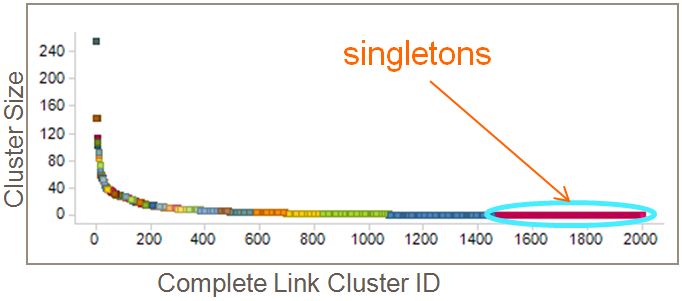
\includegraphics[width=5.5in]{fig/singletons.png}
\caption{Singletons in a complete-linkage clustering of the TCAMS dataset.}
\label{fig:platypus}
\end{figure}

Assigning each molecule to a single cluster partitions the dataset into
disparate, non-overlapping groups (also termed a hard clustering;
agglomerative fingerprint-based clustering methods such as sphere exclusion, single and complete linkage clustering\cite{Downs2003} work this way. On the other hand, a molecule could be assigned simultaneously to multiple clusters, depending on the structural features present. Traditional
hard clustering methods will not allow this and will assign such molecules
to their own cluster, thus identifying them
as singletons.  Such a result can be observed in real chemical datasets
as well -- for example, the complete-linkage clustering of the TCAMS
dataset\cite{Gamo2010,Calderon2011} has nearly 25\% of the 2000
clusters identified with just one compound, as shown in \fref{platypus}.

In contrast to hard clustering, the methods described
here rely on fuzzy clustering, where a molecule may be assigned to
multiple clusters. Fuzzy clusters have rarely been used in
cheminformatics (for example \cite{Holliday2004,Richmond2013Galois}),
perhaps because they are hard to visualize and navigate.  In this work
we provide an intuitive visualization framework for a fuzzy clustering with
multiple overlapping scaffolds per molecule. We believe this framework can help end
users easily navigate a diverse chemical dataset described by a fuzzy clustering.


\subsection{Datasets}
\label{sec:datasets}
The datasets used to illustrate and visualize our methods were picked
to represent screening datasets we expect the method to
be used on in practice. For example, the TCAMS dataset\cite{Gamo2010}
consists of 13,500 diverse hits from an antimalarial screen at GSK,
along with pIC50 against a susceptible strain of the malarial parasite
(3D7), percentage inhibition against a resistant strain (DD2), Hep G2
hepatotoxicity, a few physical chemical properties (\eg molecular
weight, aromatic ring count, cLogP), and Inhibition Frequency Index
(IFI, a measure of promiscuity defined as the percentage of screens in
which a molecule inhibits over 50\%, \cite{Chakravorty2013IFI}). The dataset is available in Ch{EMBL}'s Neglected Tropical Disease section\cite{ChEMBLNTD}.
%as file ``chemblntd\_gsk.txt.gz'' hosted as Dataset 1 on ChEMBL's Neglected Tropical Disease
%(NTD) section (\url{https://chembl.gitbook.io/chembl-ntd}), wherein each compound is identified by a Compound ID that differs from both its ChEMBL and PubChem Compound IDs. 

The in-house GSK kinase dataset shown (``Kinase X''), comprises 9259
compounds from four screening datasets for a recent kinase program.
Three of these have associated activity data from several on-target and off-target
assays: 
\begin{itemize}
\item An {\it FBDD}\cite{FBDD} (fragment-based drug design) screen run in 2011 with {\bf 288} hits.
\item A {\it full HTS} run in 2012 with {\bf 4564} {pIC50s} measured after screening 2 million compounds at a single concentration (10 uM).
\item A {\it top-up HTS} run in 2014 with {\bf 3613} {pIC50s} from screening 350,000 compounds.
\end{itemize}
A fourth dataset comprises {\bf 824} virtual compounds selected from
{\it ELT}, a DNA Encoded Library screen\cite{ELT} of 130
combinatorial libraries with billions of potential molecules.

The GSK Kinase dataset also contains physico-chemical properties of interest for
developability, notably the Property Forecast Index (PFI\cite{Young2011}). 
We chosen this dataset to illustrate the power of Scaffold Analytics in joining
and merging datasets from multiple screens, combining their SAR to
design hybrid molecules, and making inferences about unknown activity
in one screen based on known activity in another screen.

%These two and our other datasets are tabulated in \tref{dataset}, with
%references provided where available.

Next, we describe several methods we have assembled as part of our
workflow that enable multiple scaffolds to be assigned to each
molecule and easy navigation between molecules related by these
scaffolds.


%\begin{itemize}
%\item Scaffold decomposition algorithm, description
%\subitem Comparison with other decomposition algorithms
%\item Linking R-group tool to Spotfire
%\item Developing the Spotfire vis UI
%\end{itemize}
\subsection{Dataset Preprocessing}
\label{sec:prepro}
The typical dataset under consideration is available as a
comma-separated text file (CSV), whereas most of the scaffold
decomposition methods described expect MDL SD-files. To convert CSV to
SDF while preserving non-molecule fields as SDF properties, we have
created a simple workflow in Pipeline Pilot\cite{PPilot}, but this can also be done
via standard cheminformatics toolkits such as JChem\cite{JChem} or RDKit\cite{RDKit}. Prior to
SDF conversion, activity or property columns that are not to be
aggregated at the scaffold level should be deleted from the CSV file,
to accelerate analysis and aggregation.  Further quirks specific to the NCATS R-group tool
will be described in the Supplementary Material in section S3.

\subsection{Partitioning Method: Complete Linkage Clustering}
For comparison purposes, we include the default method used at GSK to visualize groups of
molecules in our visualizations. This
method produces an output file in which the unique cluster ID (CLink)
and number of other molecules in the same cluster (N\_Clink) are added
as additional fields to the original dataset.  Complete linkage
chemical clustering is described further in several references such
as \citet{Jain2010,Downs2003}.

\subsection{Fragmentation Method: NCATS R-Group Tool}
\label{sec:rgtool}
The NCATS R-group analysis tool (\url{https://tripod.nih.gov/?p=46})
was developed to automatically and exhaustively generate R-group
tables from a dataset using all scaffolds, defined as chemical
substructures shared by two or more molecules. The scaffolds are
defined as molecular fragments generated by exhaustive enumeration of
all possible combinations of the Smallest Set of Smallest Rings
(SSSR), as described at~\url{https://tripod.nih.gov/?p=160}. For a
molecule with $k$ SSSR, the maximum possible number of such scaffolds
is $2^k - 1$; however the actual number is usually much lower due to
symmetry and additional constraints (\eg reactivity, synthetic
accessibility). Briefly, the fragments are generated based on the
following rules:
\begin{enumerate}
  \item Generate Bemis-Murcko framework by iteratively pruning all foliage
    except for carbonyl (or any terminal double bond).
  \item Exhaustively enumerate all possible combinations of ring
    system. This is achieved by iteratively breaking non-aromatic
    bonds and keeping unique set of ring systems.
  \item Each fragment generated should be a valid substructure of the
    parent molecule. This constraint is approximated by ensuring the
    fingerprint for the fragment is a subset of the parent molecule.
\end{enumerate}

As an example, in \fref{scafmethod}(b) we see the five scaffolds that
were generated from the molecule shown in \fref{scafmethod}(a) from
the TCAMS dataset.

\begin{figure}
%(a)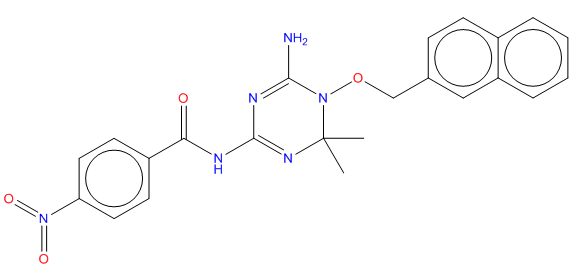
\includegraphics[width=2.5in]{fig/tcam1_mol.png}\\
%(b)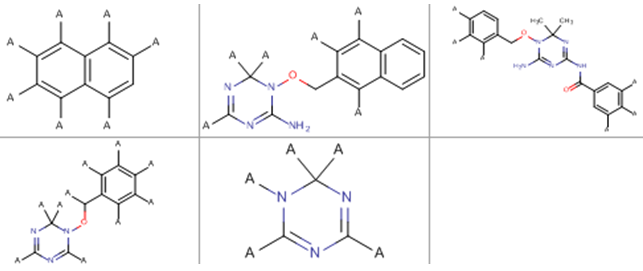
\includegraphics[width=4in]{fig/tcam1_RGscaf.png}\\
%(c)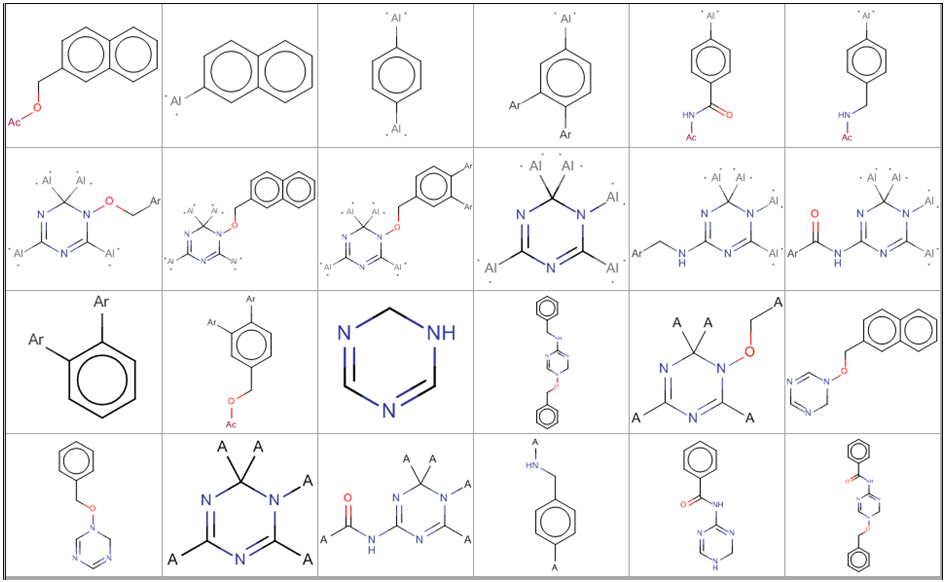
\includegraphics[width=4in]{fig/tcam1_GSKframes.png}\\
%(d)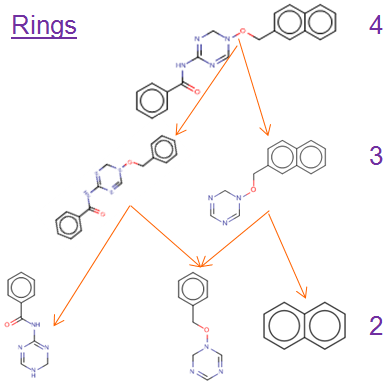
\includegraphics[width=3in]{fig/tcam1_SNG3.png}
%\caption{Scaffold Decompositions for a molecule (a) from the TCAMS dataset with PubChem Compound ID 536182. (b) 5 scaffolds from NCATS R-Group Tool; (c) 24 frameworks -- first 21 Bemis-Murcko Like and last 3 in the bottom row RECAP. (d) Scaffold Network generated by SNG, starting from top-level scaffold with four rings down to to all subscaffolds with two rings.}

(a)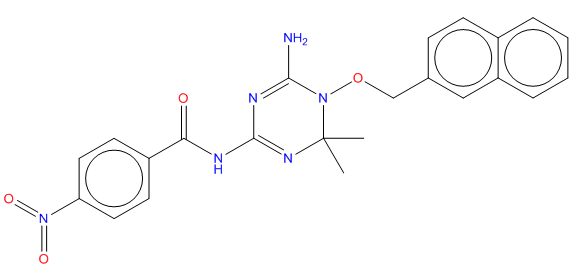
\includegraphics[width=3in]{fig/tcam1_mol.png}\\
\vspace{0.1in}
(b)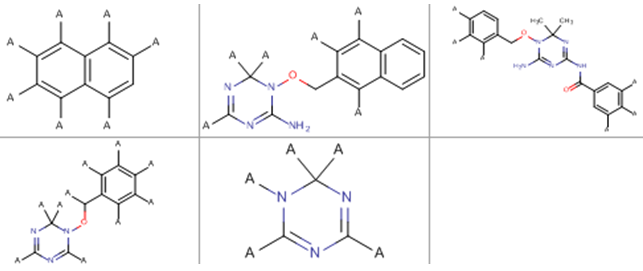
\includegraphics[width=5in]{fig/tcam1_RGscaf.png}\\
\vspace{0.1in}
(c)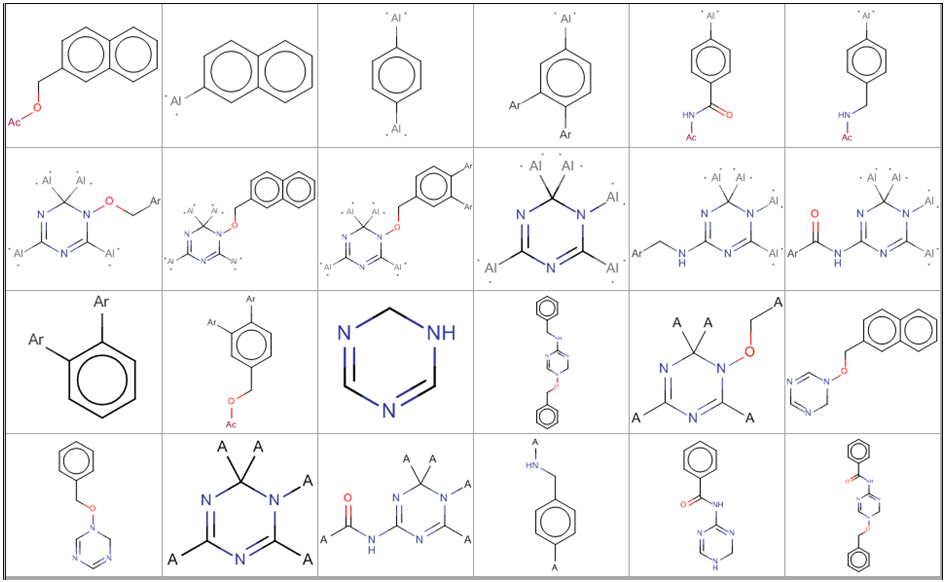
\includegraphics[width=5in]{fig/tcam1_GSKframes.png}
\caption{Scaffold Decompositions for (a) Molecule 1 from the TCAMS dataset with Compound ID 536182 (PubChem CID 44522854). (b) 5 scaffolds from NCATS R-Group Tool; (c) 24 frameworks -- first 21 Bemis-Murcko Like and last 3 in the bottom row RECAP.}
\label{fig:scafmethod}
\end{figure}


The original NCATS R-group tool focused on scaffold decomposition and
the subsequent generation of R-group tables for each scaffold. Since
then it has been extended to support scaffold hopping as well as
providing contextual data (\eg literature references, activity
summaries) and network visualizations of scaffold relationships. All
results from this study were generated in version 8 of the R-group tool,
~\url{http://tripod.nih.gov/ws/rgroupbeta/rgrouptool8.jar}). The
latest version available at time of writing is
~\url{http://tripod.nih.gov/ws/rgroupbeta/rgrouptool11.jar}), which has been
tested and produces substantially similar output.

When running from the command-line, ensuring 16G of memory (via
\texttt{-Xmx16G}) enables datasets of upto ~40k compounds with a
handful of numeric activity columns to be analyzed without running out
of memory. The scaffolds along with R-group tables for each scaffold
can be exported in a set of TSV files or a single JSON file. In the
current work we employed the TSV format which is described in detail
in Supplementary Tables S1 \& S2.

\subsection{Fragmentation Method: Frameworks}
\label{sec:gskframe}
The R-group Tool described above uses the NCATS implementation of
Bemis-Murcko Frameworks to generate scaffolds. We compare it to the
\citet{Harper2004DDclus} implementation of Frameworks.
The method generates many framework types, from which we retain two that
most resemble NCATS scaffolds for analysis: Bemis-Murcko-like\cite{BemisMurcko1996}
(with atom and bond orders retained) and RECAP\cite{Lewell:1998aa}. 

% Other fragmentation methods described by
% \citet{Harper2004DDclus} such as reduced graphs and classic
% Bemis-Murcko scaffolds (without atom types and bond orders) were
% skipped for the purposes of comparison; however there is no reason
% these could not be included in the technique we are proposing.

% the below was moved to SI.. maybe we want it back?
%The input for our implementation of frameworks is a comma separated text file
%with molecules encoded in a SMILES field.  The code was modified by
%adding scripts to export the fuzzy clusters in a tabular format rather
%than prioritize them into mutually exclusive scaffolds as in
%\citet{Harper2004DDclus}. This step produces a file similar to
%the R-group decomposition format described for the NCATS R-group tool
%in \sref{rgtool}, including the following key columns: \emph{framework
%  ID, framework SMILES, molecule ID, SMILES} and
%\emph{properties/activities}.  There are no R-group columns simply
%because this is not a default computation in our frameworks code.


The frameworks found within the same molecule from TCAMS are shown
in \fref{scafmethod}(c).  The reader will observe several differences
from the R-group tool: there are more scaffolds found, some clipped in
the middle of a linker rather than at a ring, and some redundancy
between multiple scaffolds. The current implementation does not
convert or unify tautomers among scaffolds, again leading to larger
numbers of scaffolds. % We will see in Section \ref{sec:results} that
%comprehensive coverage of fragments within each molecule can be both
%good and bad.

Further details on how we applied 
% input and output formats and how to set up and run
the frameworks code are provided in the Supplementary Material Section S4. 

%\subsection{Fragmentation Method: Scaffold Network Generator}
%\label{sec:SNG}
%The Scaffold Network Generator (SNG) \cite{Matlock2013SNG} is a
%parallelizable and robust code to generate a hierarchical Scaffold
%Network from any chemical dataset. The operation of this tool is
%described on the web at
%\url{https://bitbucket.org/swamidass/scaffold-network-generator/wiki/Home}. SNG
%takes as input either a SMILES or an MDL SD-file, and we specify
%options to generate the Network and ID Map files as two tabular
%outputs.
%
%The Network file lists each Scaffold with numeric ID, SMILES, Number
%of Rings (which serves as the level in the hierarchy) and Subscaffolds
%presented as a comma-separated numeric list. This list was converted into
%a multi-line format, one for each subscaffold, as described in the
%Supplementary Material in Section S5.
%
%The ID Map file has two columns, mapping a Molecule ID from the
%primary dataset to the Top-Level Scaffold (i.e. Murcko scaffold)
%obtained by stripping all pendant groups but no rings. Using the ID
%Map file followed by multiple iterations of the Network file one can
%elucidate the entire Scaffold Network starting from each query
%molecule, as described in a subsequent section.  As an example the
%scaffold network generated for a molecule from TCAMS is shown in
%\fref{scafmethod}(d), as for the previous two methods.


\section{Methods: Data Integration and Visualization in Spotfire}
\label{sec:methods2}

Next, we describe how tabular scaffold output generated using the
NCATS R-group tool and other comparable methods is integrated into
Spotfire, a visualization tool of choice at many companies. 

\subsection{Data Table Generation and Linking}

\begin{figure}
%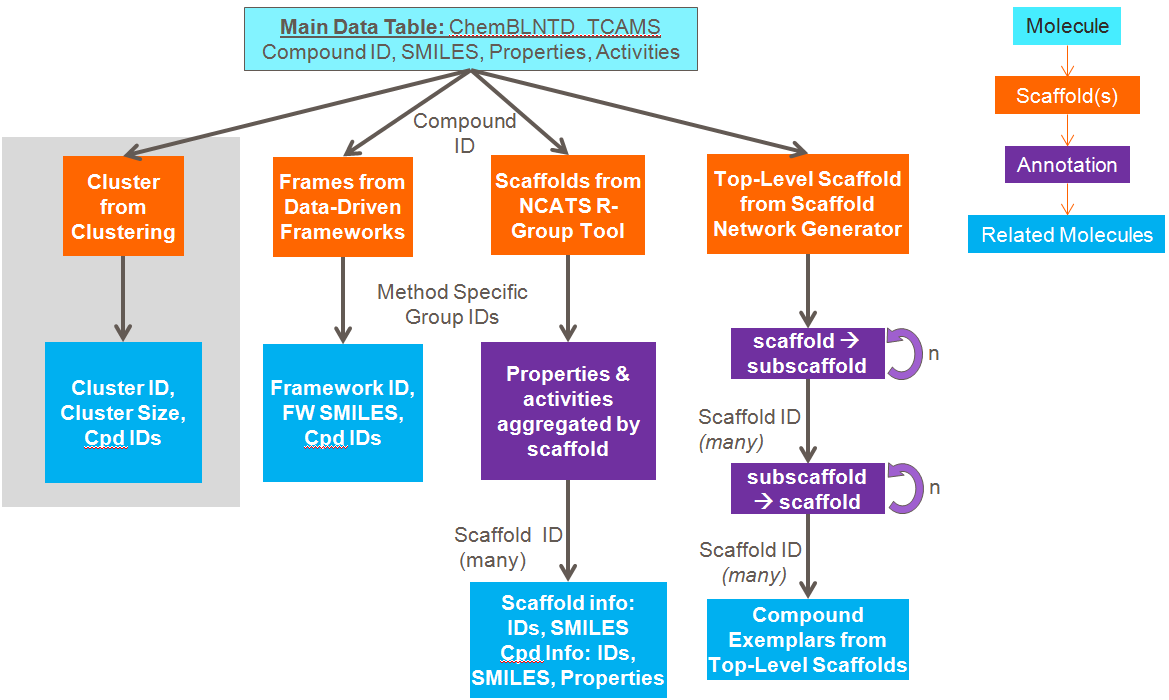
\includegraphics[width=6in]{fig/details_all2.png}
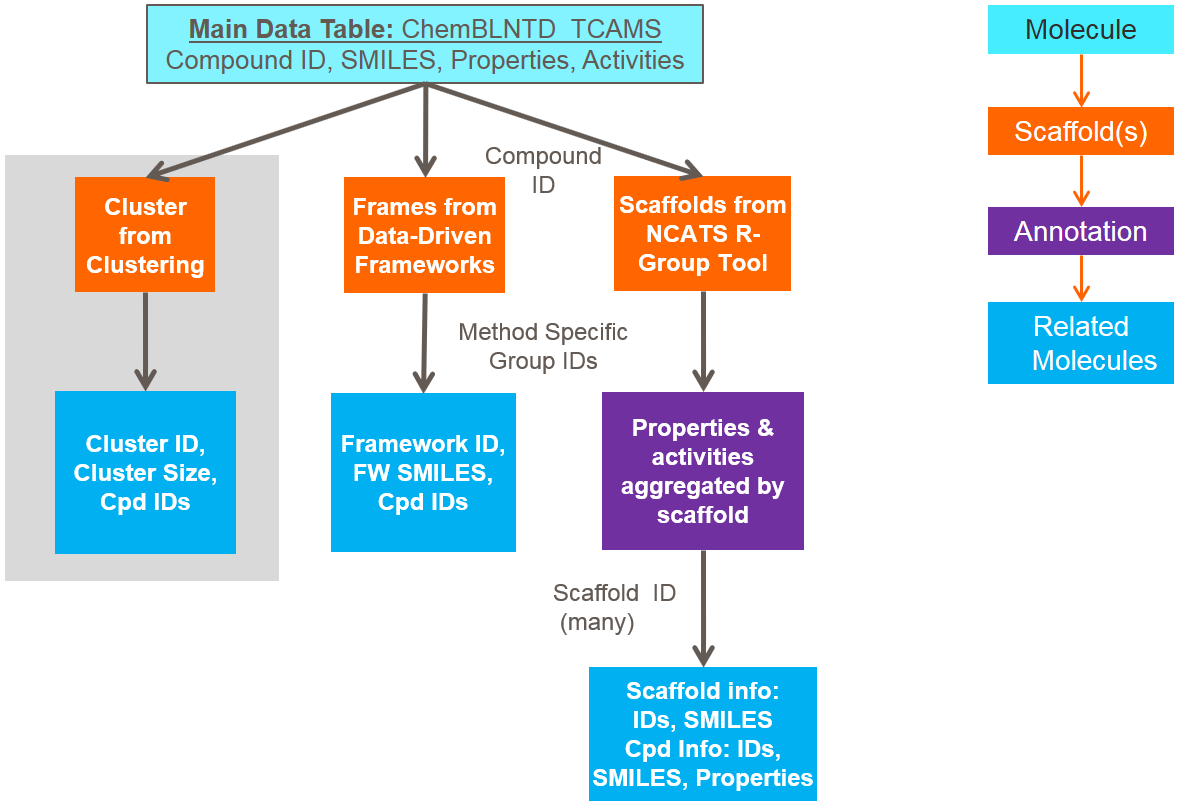
\includegraphics[width=6in]{fig/details_all3_noSNG.png}
\caption{Detailed schematic on how the output from clustering and
  fragmentation methods are set up as data tables and linked together
  with the main dataset in Spofire. Right inset: schematic color-coded
  view of the scaffold-walking navigation that is loosely followed in
  this diagram.}
\label{fig:detaildevil}
\end{figure}

\fref{detaildevil} shows how the data tables output by the scaffold
generation methods considered here are layered onto the primary data
table in Spotfire. This primary data table is usually a direct database
import of tabular molecule and activity data or available from public
datasets. What gets added follows the schema ``Molecule --> Scaffold (including Annotation)
--> Related Molecules'' shown in the figure. For each Molecule in the
dataset, we connect it to every Scaffold/Framework/Cluster it
contains, and then to every other molecule containing any of these
Scaffolds/Frameworks/Clusters. Slight differences for each individual
method are detailed in the Supplementary Material, Section S6.

\subsection{Visualization of Molecules, Scaffolds and Related Molecules}

We next describe a minimalistic user interface for exploring the
network of molecules, the scaffolds they contain and related molecules
that contain the same scaffolds. This interface consists of the
following elements:
\begin{itemize}
\item {\bf Main Window}: Views defined that allow one to explore the
  Primary Data Table (with no scaffold information) in the most interpretable
  way for each dataset.  In the canonical example, key activity,
  selectivity, ligand efficiency and molecular properties may be
  highlighted on the X, Y, shape, size and color axes on a scatter  plot.
  This view is depicted in compressed form in the top half of \fref{spotviz}(a).
\item {\bf Related Molecules Tab}: The purpose of this tab is to
  implement the Scaffold Walking navigation described briefly earlier.
  The setup is described for the NCATS R-group Tool decomposition,
  though this tab applies to and can be set up analogously for any
  other decomposition. The tab consists of two visualizations,
  illustrated for the TCAMS dataset in \fref{spotviz}(a): \subitem The
  first one is a miniature version of the Main window, allowing the
  user to select (in Spotfire, mark) molecules of interest without
  flipping over to the Main tab. Doing so drives one of the following
  two Details Visualizations on the {RG}decomp table, showing only
  molecules from the scaffolds contained in the marked molecule, \ie
  Related Molecules: \subitem {\bf Scaffold Trellis}: This scatter
  plot is trellised by Scaffold ID and ideally displays the same
  properties on the axes as the Main visualization above it.  An
  example is shown in \fref{ELT}. The trellis allows us to break up
  the SAR for each constituent scaffold individually, identifying
  promising scaffolds and substituting unproductive ones as we will
  describe in the Discussion. The trellis visualization suffers from
  redundancy: the same molecule occurs in multiple trellis panels and
  the only way to link them is by X and Y coordinates, by observing
  groups of points that are laid out similarly across multiple trellis
  panels.  Though some of our users still prefer this approach, we now
  describe a newer solution that better leverages Spotfire's
  capabilities.  \subitem {\bf Scaffold Pies}: Instead of using a
  trellis, the Marker shape is changed to Pies, with Colors (which map
  to pie sectors) by Scaffold ID, and sectors sized by the Count of
  molecules in each scaffold.  The result is illustrated in
  \fref{spotviz}(a). This plot shows only one point per related
  molecule but one sector for each scaffold it shares with the parent
  molecule.  As described in Section \ref{sec:results}, this lets the
  user quickly and visually home in on key substructures that are
  important or unimportant for activity.

\item {\bf Scaffolds and R-groups Tab}: This tab, currently specific to the NCATS R-group tool method for generating scaffolds, contains two visualizations, as illustrated for the TCAMS dataset in \fref{spotviz}(b)--(c):  
  \subitem The first is a scatter plot display of the Scaffolds table, displaying scaffold Complexity and Count and aggregate activity of each scaffold either on the axes or using the Size and Shape dimensions.  Here scaffolds of lesser interest (for example with low complexity or count) can be identified and tagged to remove them from the analysis. Conversely, scaffolds of high interest, for example with many active members or high aggregate ligand efficiency, may be tagged into separate categories.
\subitem The second plot is an R-group table, \ie a Table view of the {RG}decomp table limited to data records that have been marked, \ie molecules that lie in scaffolds currently marked. The table is sorted first by scaffold and then by primary activity, and molecular fields such as Scaffold SMILES, Molecule SMILES and R-groups $R\_1..R\_n$ are rendered using an appropriate depiction package - at GSK this is {JChem}\cite{JChem}.  This table may be exported to Excel as an on-the-fly R-group table of the scaffolds of interest.

\end{itemize}

\begin{figure}
(a)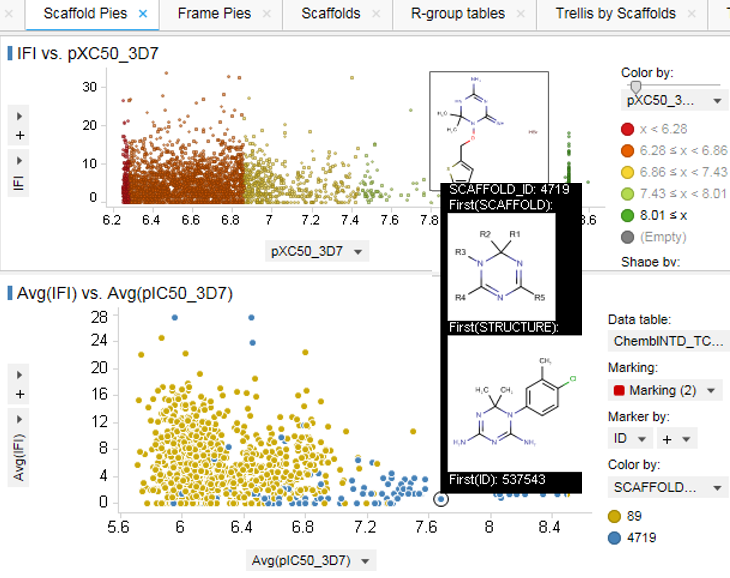
\includegraphics[width=5in]{fig/spotviz_scafpie_tooltip.png}\\
(b)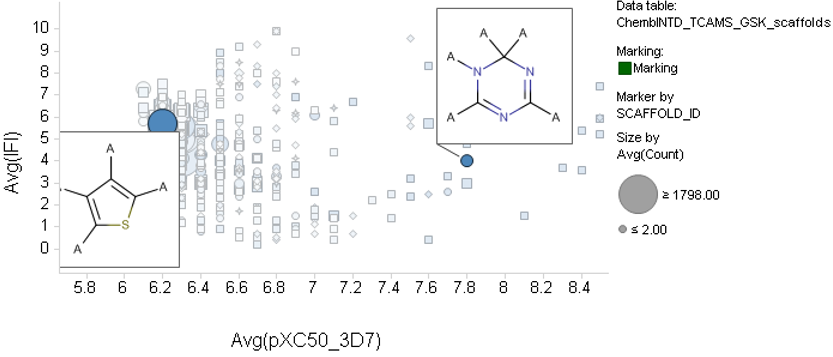
\includegraphics[width=5in]{fig/spotviz_scaffolds_aggr.png}\\
(c)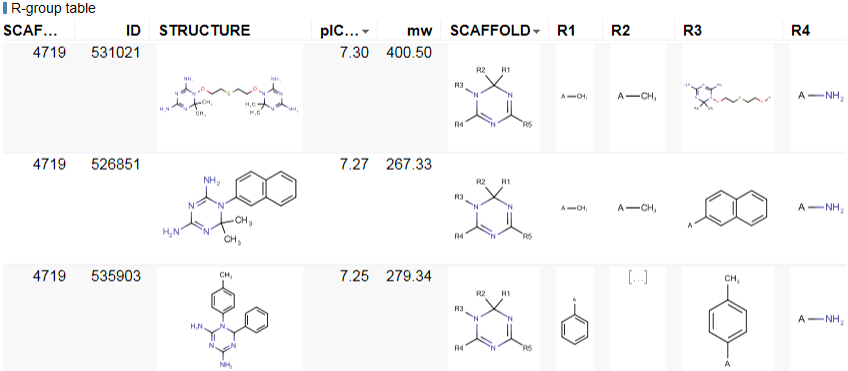
\includegraphics[width=5in]{fig/spotviz_RGtable.png}
\caption{Elements of the minimal Spotfire interface we developed for Scaffold-Based Analytics: (a) Related Molecules page, with molecule selection in the top panel and related molecules viewed as one pie sector per scaffold shared; (b) Aggregate plot of scaffold statistics (with often a detailed drill-down into the selected scaffold);  (c) R-group table on selected scaffolds, sorted by scaffold ID and decreasing pIC50 or other desired properties.}
 \label{fig:spotviz}
\end{figure}

Alternative visualizations are possible and we describe some of them
in the Supplementary Material, Section S7. In addition, we discuss several
Spotfire tricks that are instrumental in making our visualization
useful to the chemist or biologist
user. %\textbf{\textcolor{red}{TODO}}

\subsection{Statistical Comparison of Scaffold Generation Methods}
\label{sec:statmethod}
In this section we define the statistical methods used to compare the
scaffold generation methods in the context of annotating molecules in
a screening dataset with multiple, possibly overlapping scaffolds (as
opposed to partitioning the set of molecules into non-overlapping
categories, a.k.a. clustering). The code to implement these methods is released
as part of the Supplementary Material in Section S8.

The similarities and differences between non-overlapping clusterings
have been analyzed in the literature, and one example is the method of
\citet{Torres2009}, who provide a similarity measure between
outputs of two partitioning clustering methods. They use Jaccard's
similarity coefficient $S_{ij}$, defined as the ratio of intersection
size to union size of two groups $i$ and $j$ in the clustering.  This
coefficient, computed pairwise and summed, yields a simple similarity
measure between two clusterings $X$ and $Y$ with $m$ and $n$ clusters,
respectively:
\begin{equation}
Sim(X,Y) = \Sigma_{i \le m, j \le n}{S_{ij} / max(m,n)}
\end{equation}

We adapt this method for SAR analysis using overlapping scaffolds,
where the question on the minds of chemists is twofold: what are the
fragments in active/desirable molecules, and which other molecules
share these fragments? Given two fragmentation schemes, $A$ and $B$,
we can evaluate for any molecule how many other molecules share
fragments using $A$ or $B$, and thus can be found using fragmentations
$A$ alone, $B$ alone, $A$ and $B$, or $A$ excluding $B$.  Using these
methods we can evaluate the overall similarity of the two
fragmentation schemes, and also independently score the usefulness of
$A$ and $B$ to connect compound(s) of interest to related molecules. 

For any compound $C$ and fragmentation $A$, define the structure group of
$C$ under $A$, $C_A$ as the set of compounds that share fragments from
$A$ with compound $C$. Similarly define the structure group of $C$
under $B$, $C_B$ as the set of compounds that share fragments from
$B$. The Common Proportion ($CP$) for compound $C$ is then defined as
the ratio of the number of compounds common to $C_A$ and $C_B$ to the
total number of unique compounds contained in $C_A$ and $C_B$:
\begin{equation}
CP_{A,B}(C) = \| C_A \cap C_B \| / \| C_A \cup C_B \|
\end{equation}
Similar statistics can be defined to rank the usefulness of an
individual fragmentation given others. The Proportion of Information
$PI_A$ calculates the proportion of compounds reachable from $A$ and
$B$ that would be reachable from $A$ alone:

\begin{equation}
PI_A(C) = \| C_A \| / \| C_A \cup C_B \|
\end{equation}

In constrast, the Proportion of Information Unique to $A, PIU_A$ uses the set difference between $C_A$ and $C_B$ to get at the question: if I have $B$, do I still need $A$? 

\begin{equation}
 PIU_A(C) = \| C_A \setminus C_B \| / \| C_A \cup C_B \| = 1 - PI_c(B)
 \end{equation}
  
 When comparing one fragmentation method against another, we often see
 that one method utilizes a larger number of shared fragments than the
 other in order to connect compound $C$ to a very similarly sized
 structure group. To capture this tendency and reward methods that
 connect molecules to related ones efficiently rather than
 exhaustively, we define a Fragment Efficiency measure as follows. Let
 $frag_A(C)$ be the set of fragments of compound $C$ in fragmentation
 $A$ that connects $C$ to its structure group $C_A$. Similarly define
 $frag_B(C)$ for fragmentation $B$. Then:
\begin{equation}
FragEff_A(C) = \| C_A \| / \| frag_A(C) \|
\end{equation}


These statistics can be averaged over all compounds in a dataset to
yield the Average Common Proportion (ACP), Average Proportion of
Information (API), Average Proportion of Information Unique to A
(APIU) or Average Fragment Efficiency (AFE).  Other statistics can
also be applied to the distribution of $CP$, $PI$ or $PIU$ to
characterize the dataset and overlapping scaffolds used to
characterize it.

Our methods extend the similarity score of \citet{Torres2009} to
overlapping clusters by using a set of clusters derived from them,
defined as follows:
\begin{itemize}
\item Replace the original clusters by new clusters, one for each item
  in any cluster (in this case, any compound in the dataset).
\item The cluster for Compound $C$ contains all compounds that appear
  with Compound $C$ in any cluster, \ie $C_A$.
\end{itemize}


\section{Results}
\label{sec:results}
Here we illustrate some of our key findings and use cases on a few datasets. 

\subsection{Use Case: Scaffold Progression and Prioritization}
Aggregate statistics such as maximum, minimum, mean and standard
deviation, computed at a per scaffold level, may be useful in
prioritizing scaffolds. For example, \fref{RGTaggr} shows the six
scaffolds contained within a tricyclic molecule (Molecule
2, TCAMS Compound ID: 541564, PubChem CID: 44531725)
ranked by average activity and IFI. This ordering may
be used to determine which substructures are most important for the
molecule's activity, and use this information to design or test
further compounds.

\begin{figure}
  (a)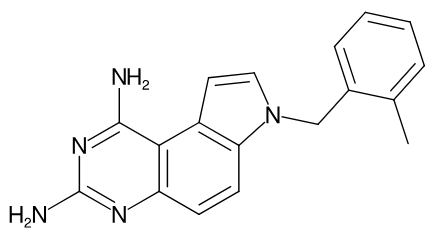
\includegraphics[width=2in]{fig/tcam2_mol_541564.png}
  (b)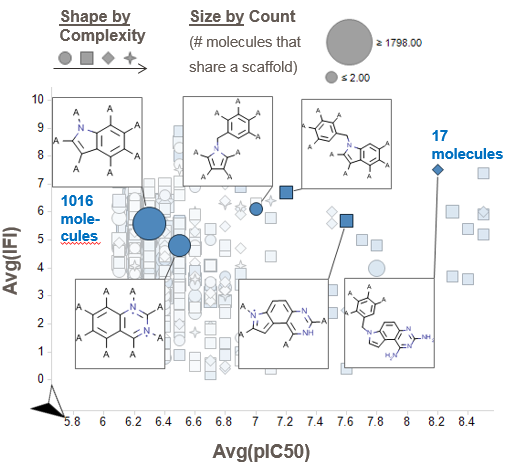
\includegraphics[width=5in]{fig/RGT_aggr_prop2.png}
  \caption{(a) Molecule 2 (TCAMS Compound ID: 541564; PubChem CID: 44531725).
    (b) All \~5000 scaffolds from the TCAMS dataset ranked by
    average pIC50 in the P.~falciparum 3D7 strain and Inhibition
    Frequency Index. The six scaffolds contained in Molecule 2
    are shown in increasing order of average pIC50.}
\label{fig:RGTaggr}   
\end{figure}

For the in-house kinase dataset, the program team were looking for hit series with activity in a range of orthogonal on-target assays, selectivity against a mutant counter-screen, and good properties to predict developability.  We aggregated the activity in each of the primary assays, selectivity, and Property Forecast Index (PFI~\cite{Young2011}), using the mean values as filters to identify promising scaffolds.  A plot of aggregate selectivity \vs PFI is shown in \fref{KinaseX}(a).

Once a promising scaffold is identified, one can drill down with a single click into detailed activities and properties of the molecules containing the scaffold to decide whether to pursue the series further. For example, the
the scaffold with ID 2988, marked in \fref{KinaseX}(a) has on the aggregate good selectivity (1.4 log units) and also low PFI (6.7). The activity profiles for 8
molecules sharing this scaffold are shown in \fref{KinaseX}(b). Clear differentiation is observed between an orthogonal suite of native protein assays and the mutant assay, marking the scaffold as a good one to explore making additional molecules.

\begin{figure}
  (a)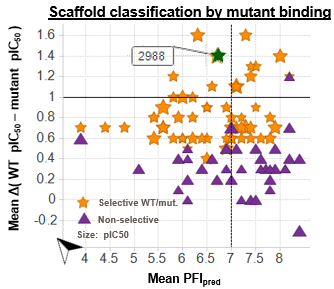
\includegraphics[width=5in]{fig/KinaseX_RG_aggr.png}\\
  (b)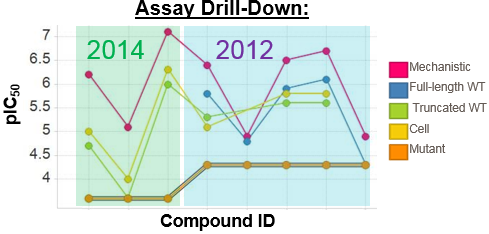
\includegraphics[width=5in]{fig/KinaseX_RG_drill.png}
  \caption{(a) Aggregate scaffold statistics for molecules from the Kinase X dataset, with average selectivity against a mutant assay in log units on the Y-axis and average PFI (Property Forecast Index) on the X-axis.  Scaffolds are tagged as selective or non-selective after exploring their detailed properties. (b) Detailed properties of 8 molecules that share scaffold 2988 (structure not shown), split over two HTS datasets from 2014 and 2012. Lines are color-coded by assay type, and the mutant assay is shown in orange across the bottom of the graph.   
  }
\label{fig:KinaseX}   
\end{figure}


To conclude, we have observed how scaffold-based analytics allows us to make decisions based on the aggregate (average, SD, median, min, max, ...) properties of molecules in scaffolds. An entire scaffold may be rejected or prioritized at a time instead of keeping track of individual molecules. It is important to note that rejecting a scaffold does not reject all molecules containing that scaffold - otherwise rejecting the benzene ring would remove a large percentage of valid leads.
%Also at any time we are able to drill down into the data for individual compounds in interesting scaffolds, whether in an R-group table or a custom plot, and incorporate that into our prioritization.   

\subsection{Use Case: Dataset Fusion and Hybridization}
In the previous section and \fref{KinaseX}(b), we noted that the 8 molecules sharing scaffold 2988 came from two datasets, \viz HTS hits from 2012 and 2014. This is significant since the 5 molecules found during the 2012 campaign were not prioritized since they did not jump to the top using visual inspection, clustering or other methods used to triage the hits -- this Scaffold-Based Analytics method was not available. However, when the hits from both screens were combined and analyzed with this method in 2014, the pattern of activity, selectivity and properties that made these desirable hits to pursue was automatically found and readily flagged.

In this way, Scaffold-Based analytics may be used to combine multiple datasets using the scaffold as the common unit of comparison and merging, with dataset labels identifying molecules in the resulting merged dataset. If the datasets have comparable activities, as the Kinase X HTS datasets did, aggregate statistics are easy to compute. If they do not, \eg if one dataset has $pIC_{50}$ and others primary screening activity or a different measure of desirability, normalized activities may be computed to enable aggregation at the scaffold level.

Sometimes one of the datasets does not contain activities at all, \eg
in the case of virtual molecules from a DNA Encoded Library Technology\cite{ELT}
(ELT) screen, or for molecules from a vendor catalog that are yet to
be ordered and assayed. In \fref{ELT} we show an example where two
computed properties, Molecular Weight and PFI were used to identify
promising virtual molecules from the ELT dataset to make, and untested
molecules from the FBDD\cite{FBDD} (Fragment-Based Drug Design) dataset to test.

\begin{figure}
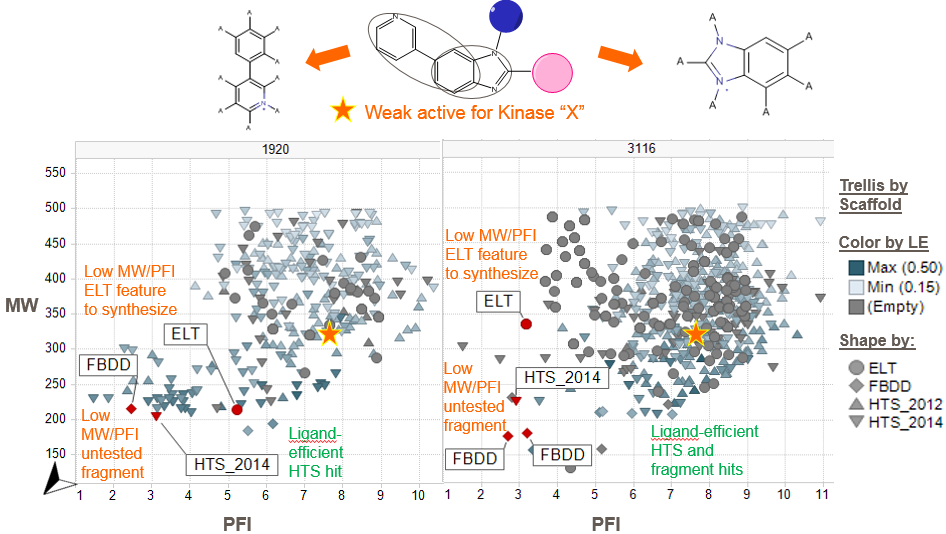
\includegraphics[width=6in]{fig/KinaseX_ELT.png}
\caption{
Two scaffolds with ID 1920 (pyridophenyl) and 3116 (benzimidazole) shown in a trellised plot of molecules related to a weak active in the Kinase X 2014 HTS screen. The axes of the plots are computed properties, MW and PFI, to allow molecules without measured activity or virtual molecules not yet synthesized to be included in the plot. The compass arrow device points in the direction of improved properties -- lower MW and PFI. Interesting related molecules are labeled on the plot, including untested fragment-like molecules from the FBDD dataset, virtual molecules from the ELT dataset, and another ligand-efficient hit from the HTS2014 dataset, all with low MW/PFI. The unmeasured and unmade molecules are good candidates for future synthesis and testing.   
}
\label{fig:ELT}   
\end{figure}


\subsection{Use Case: Scaffold Walking Navigation}
\label{sec:scafwalk}
Scaffold Walking is our term for navigating from molecule(s) through scaffolds (implicitly) to Related Molecules. This contrasts with Scaffold Hopping, which is usually defined as a complete replacement of a scaffold by another 2D-dissimilar but 3D-similar or bioisosteric scaffold. Scaffold Walking is meant to be a gradual change to the molecule, at each step retaining at least one element of its maximal Murcko scaffold (\ie at least one among the multiple scaffolds it shares with other molecules in the dataset).  In the process the SAR gets deconvoluted in terms of these scaffolds, allowing us to determine visually both the most essential scaffolds in a molecule and the best Related Molecules containing them.       
\begin{figure}
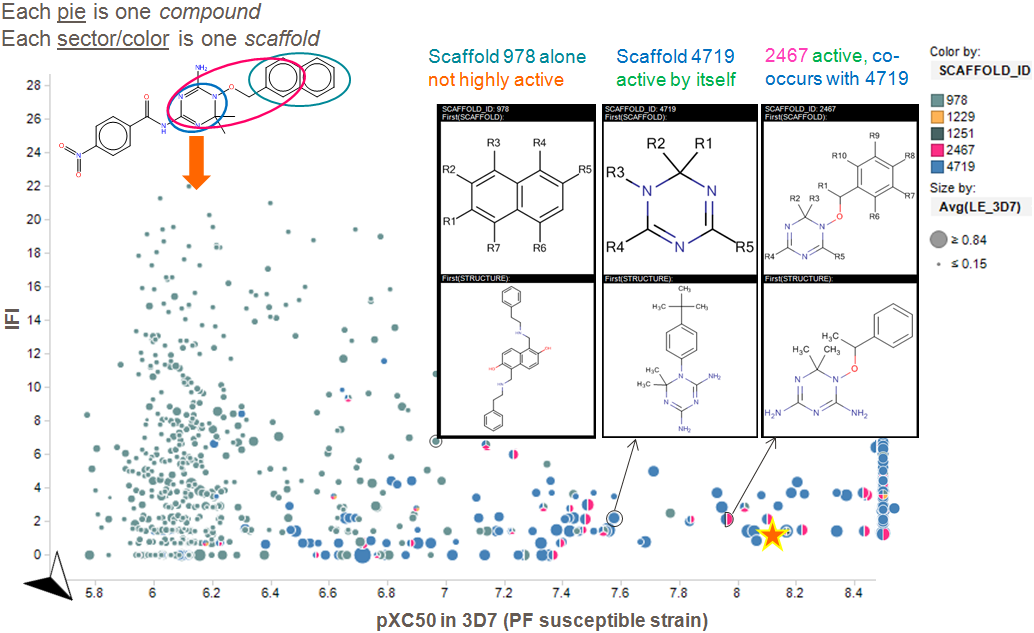
\includegraphics[width=6in]{fig/mol1_RGtool_scafpie.png}
\caption{Related Molecules scaffold pies visualization for Molecule 1 (TCAMS Compound ID: 536182, PubChem CID 44522854). Each pie here is one related molecule, and each pie sector and color is a scaffold that it shares with the parent molecule. The star symbol is added to show the location of the parent molecule in this plot, and the compass device at the origin shows the direction of favorable properties (in this case towards the +X and -Y axes). Insights derived from the plot are highlighted in the figure and also discussed in the text.}
\label{fig:scafwalk1}
\end{figure}

As an example, consider Molecule 1 (TCAMS Compound ID: 536182, PubChem CID 44522854) in \fref{scafwalk1}, as a hit that we want to explore SAR of and optimize. This molecule contains 5 scaffolds as determined by the NCATS R-group tool. Using the Scaffold Pie visualization, we observe that the naphthyl scaffold (\#978, cyan) is by itself only moderately active.  The dihydrotriazine (\#4719, blue) scaffold is observed to always occur where the dihydrotriazine-phenethyl-ether (\#2467, pink) one does, implying the substructure relationship between them visually even if one did not know it beforehand. Scaffold \#4719 also exists and is active without \#2467, implying that the phenethyl ether can be substituted and the dihydrotriazine may be sufficient for activity by itself.

\begin{figure}
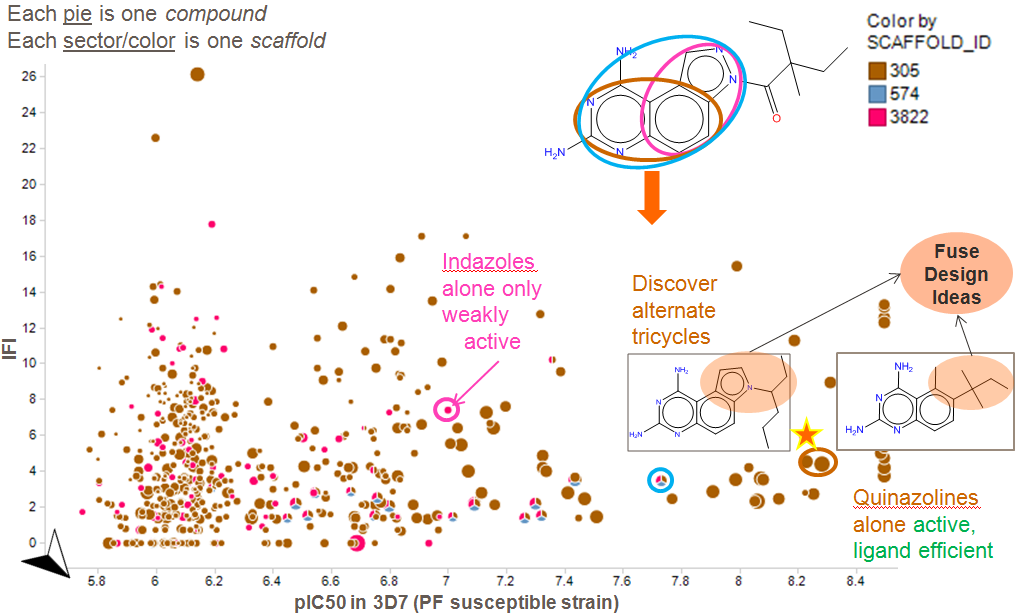
\includegraphics[width=6in]{fig/mol2_RGtool_scafpie2.png}
\caption{Related Molecules scaffold pies visualization for Molecule 3 (TCAMS Compound ID: 533945; PubChem CID: 44531163). Each pie here is one related molecule, and each pie sector and color is a scaffold that it shares with the parent molecule. The star symbol is added to show the location of the parent molecule in this plot, and the compass device at the origin shows the direction of favorable properties (in this case towards the +X and -Y axes). Insights derived from the plot are highlighted in the figure and also discussed in the text.}
\label{fig:scafwalk2}
\end{figure}

Molecule 3 in \fref{scafwalk2} is another case where we might want to optimize the physical and chemical properties of the molecule without sacrificing activity or increasing promiscuity. Since solubility has been shown to decrease with number of aromatic rings independent of lipophilicity\cite{Hill2010}, walks that remove one or more of the three fused rings might be beneficial. By exploring the Related Molecules, we observe the SAR for three scaffolds: quinazolines (\#305, brown), indazoloquinazolines (\#574, blue) and indazoles (\#3822, pink). We observe from the plot a few more molecules containing all three scaffolds (tricolored pies, \ie exact analogs of the parent molecule); all of these are less active than the parent. The indazoles when they occur alone (pink circles) are far less active than the parent, suggesting they do not contribute significantly to activity and may be substituted. Lastly the quinazolines (brown) include several analogs that are more active and also less promiscuous than the parent. Drilling down into these structures, we observe several that contain only two aromatic rings (\ie no more are either fused or attached); these provide novel, active and ligand-efficient templates on which to build new analogs with enhanced solubility or other properties. Suggestions for which analogs to make can often be obtained by examining the SAR -- for example, disparate aliphatic and aromatic analogs at two adjacent positions on the quinazoline phenyl are active, which suggests hybridizing them or designing further analogs substituted at these positions.

\begin{figure}
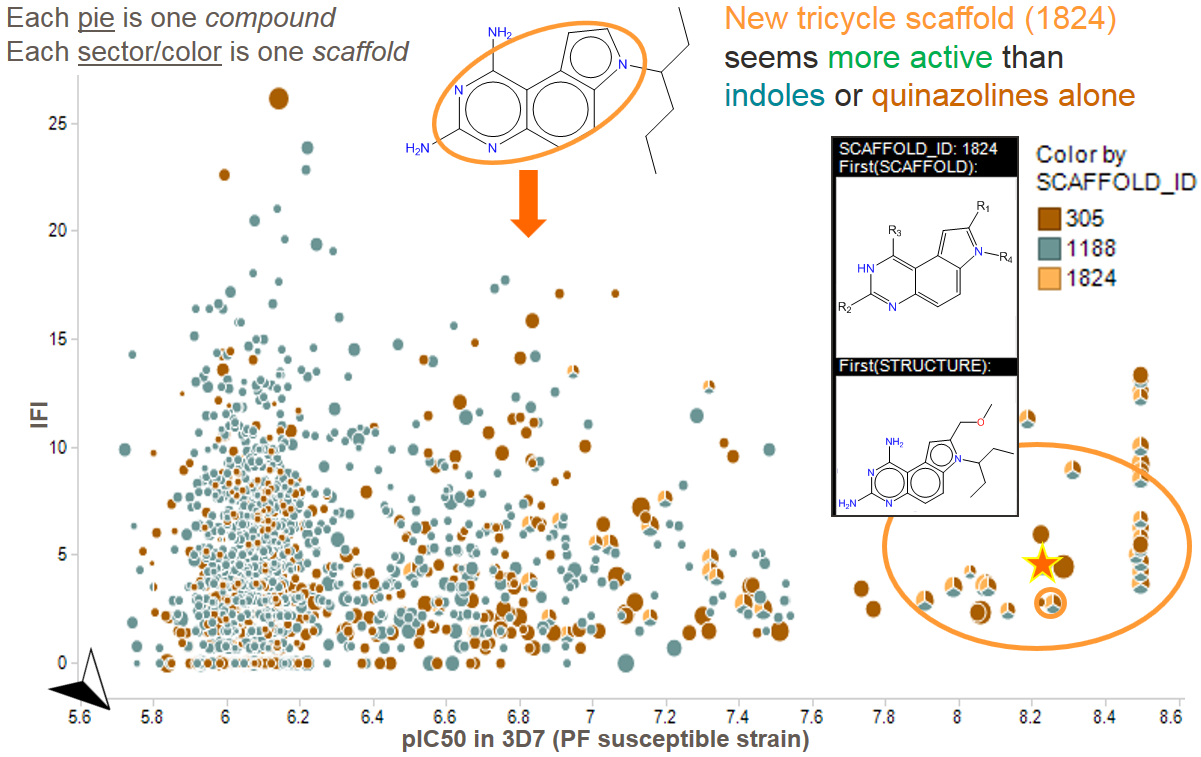
\includegraphics[width=5.5in]{fig/mol3_RGtool_scafpie_iter.png}
\caption{Iterative Related Molecules scaffold pies visualization for Molecule 4 (TCAMS Compound ID: 541531, PubChem CID: 44531903), a scaffold hop from Molecule 3 shown in \fref{scafwalk2}. Each pie here is one related molecule, and each pie sector and color is a scaffold that it shares with the parent molecule. The star symbol is added to show the location of the parent molecule in this plot, and the compass device at the origin shows the direction of favorable properties (in this case towards the +X and -Y axes). Insights derived from the plot are highlighted in the figure and also discussed in the text.}
\label{fig:scafwalk3}
\end{figure}

Another intriguing result is seen by observing a new tricyclic series that shares the quinazoline but adds an indole instead of indazole as the third fused ring. This alternative tricyclic template, while it may not confer solubility advantages, opens up a new area of chemical space. By iteratively seeking the Related Molecules for this new hit as shown in \fref{scafwalk3}, we observed that most of the active quinazoline analogs have this new tricyclic scaffold (\#1824, tan wedges in tricolored pies) and relatively few contain only quinazolines (\#305, brown circles). Also, indoles by themselves (\#1188, blue circles) do not much better than indazoles, so this is a new synergistic effect discovered by scaffold walking from the original hit.            


\subsection{Qualitative Comparison of Scaffold-Generation Methods and Clustering}
{\bf Complete-Linkage Clustering}: As shown in \fref{clusterlanes}, the defining feature of a partitioning clustering is that every molecule maps to one and only one cluster. Thus if a chemotype is broken up among two or more clusters, using the cluster ID to map Related Molecules can retrieve only neighbors from the same cluster, ignoring the other cluster. This is not ideal for purposes of the visualization and navigation method presented here, as arbitrary neighbors would be excluded depending on how the clustering is defined.  Thus we do not advocate the use of clustering, unless it is a fuzzy clustering where all meaningful class memberships a molecule might have are considered. 

\begin{figure}
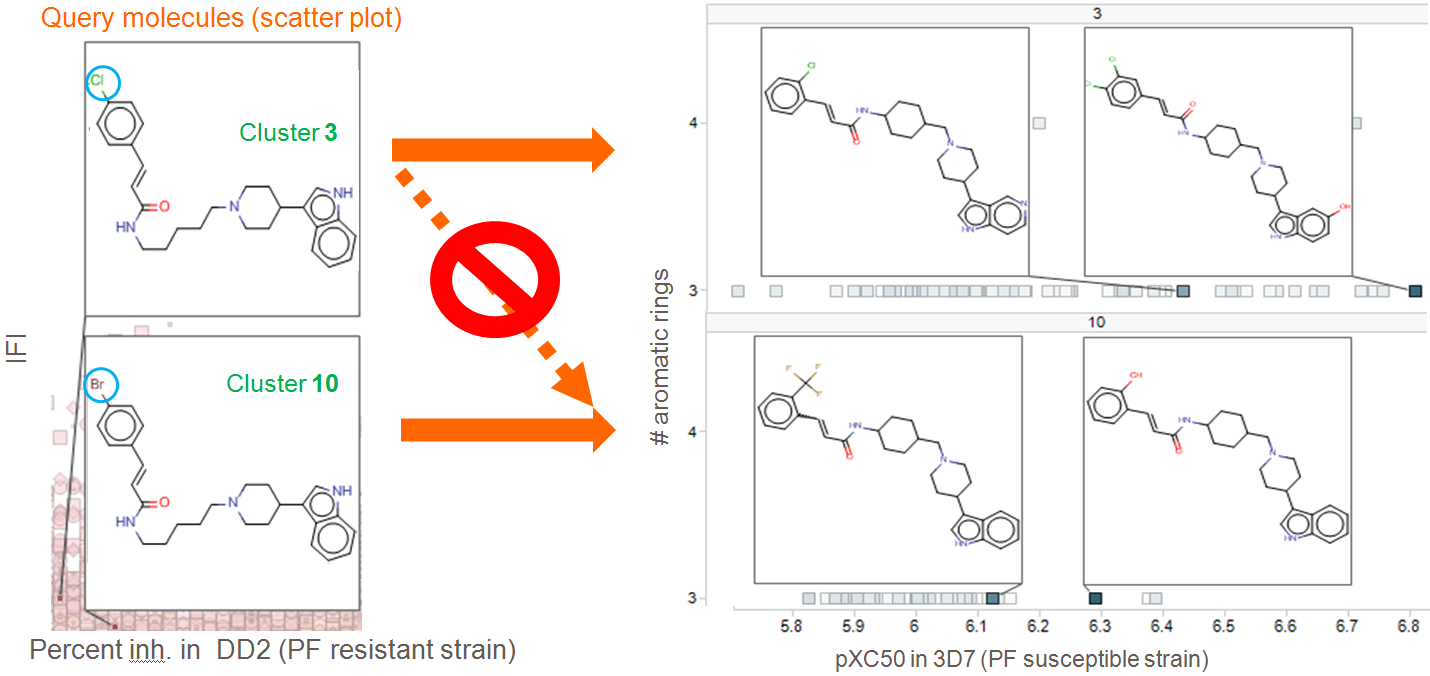
\includegraphics[width=6in]{fig/clusterlanes.png}
\caption{Illustrating one problem with clustering: bifurcation of related molecules.  When two molecules of the same chemotype differing by a halogen are split across Complete Linkage Clusters, searches of cluster neighbors for one molecule do not find its analogs in the other cluster, \ie the two related clusters are not linked.}
\label{fig:clusterlanes}
\end{figure}



{\bf NCATS R-group tool}: As opposed to the clustering method, 
if any two molecules share a common substructure that meets the standards required of a scaffold by the NCATS method (\eg being bordered by rings on each end), then those molecules will be found to contain that shared substructure as a scaffold and their activities will be used to compute aggregate properties for it. 

{\bf Other Scaffold Generation Methods}: As shown earlier, even though another scaffold generation method (represented here by the \citet{Harper2004DDclus} implementation of Frameworks) differed in its implementation details and produced different numbers of scaffolds for the same molecule, it was roughly equivalent in a qualitative sense with regard to the insights obtained. Due to substantial overlap between sets of scaffolds, ring systems responsible for activity of a molecule were generally revealed by either method. For example, the insights mentioned in \sref{scafwalk} were more or less consistent across the methods. However, there were cases where the Frameworks revealed negative information about a fragment being not important for activity that is also useful for a drug discovery scientist. For example, in \fref{frameswalk} a substructure is highlighted that is on the aggregate inactive and could be removed or substituted. This insight is not available from SSSR-based scaffolding methods such as the NCATS R-group tool since they don't define or find that fragment as a scaffold.

\begin{figure}
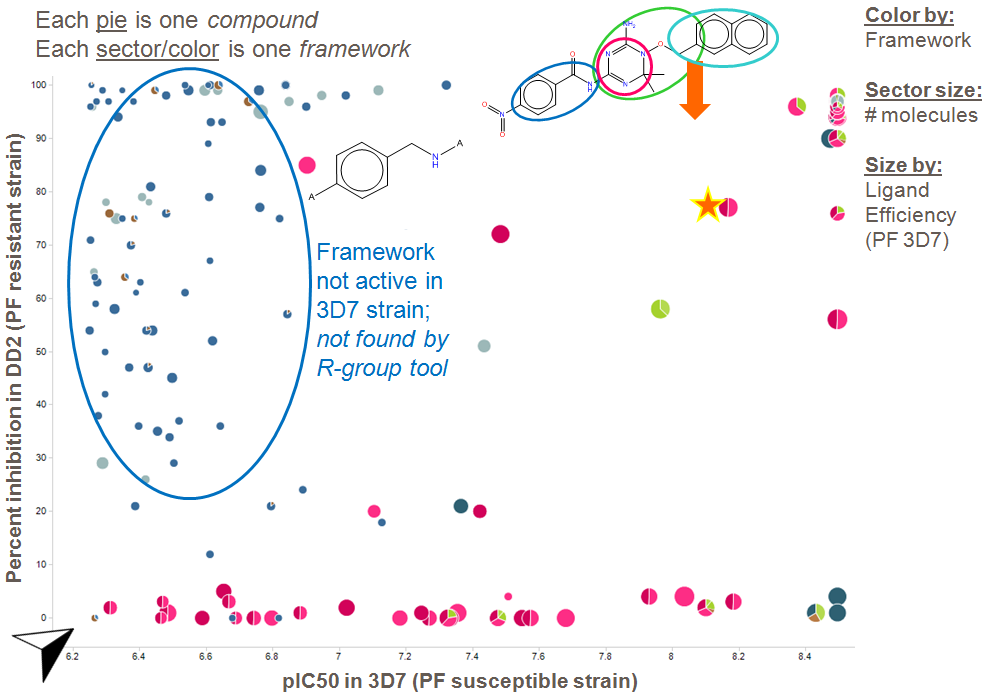
\includegraphics[width=5in]{fig/mol1_frames_scafpie.png}
\caption{Using Frameworks with the Scaffold Pies visualization. One framework is highlighted that has no equivalent in the NCATS scaffolds, but is shown to reduce activity as related molecules containing it are less active than the parent molecule.   The star symbol shows the location of the parent molecule in this Related Molecules plot, and the compass device at the origin shows the direction of favorable properties (+X and +Y axes).}      
\label{fig:frameswalk}
\end{figure}


To summarize, both multiple-scaffold decomposition methods considered in this study, \ie NCATS R-group Tool and Frameworks give comparable insights when exploring the TCAMS dataset, with some differences stemming from individual substructures that are considered shared scaffolds or not by the individual methods.  We now explore these overlaps, similarities and differences in the aggregate using the statistical methods described earlier in \sref{statmethod}.


\subsection{Statistical Comparison of Scaffold-Generation Methods}\label{sec:statcomp}

Recall the concepts of structure group and common proportion defined in \sref{statmethod}.  Let us now apply these to analyze and compare the scaffold generation methods Frameworks ($A$) and NCATS R-group tool ($B$). As an illustration, \fref{strucgroup} (a)-(c) shows the structure group of the compound $C$ with Compound ID 541564 (PubChem CID: 44531725). 
\begin{figure}
\centering
  \begin{minipage}[b][0.2\textheight][s]{0.3\textwidth}
  \centering
  (a)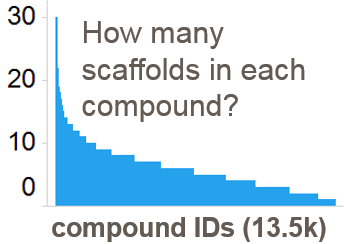
\includegraphics[width=1.5in]{fig/howmany_scaf.png}
  (b)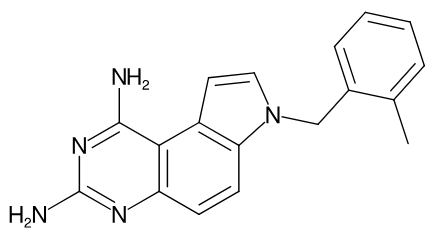
\includegraphics[width=1.5in]{fig/tcam2_mol_541564.png}
  \end{minipage}
  (c)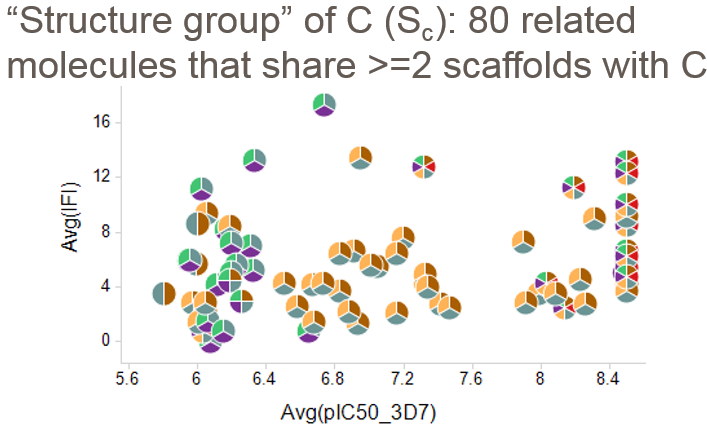
\includegraphics[width=3in]{fig/structure_group_C.png}
  %%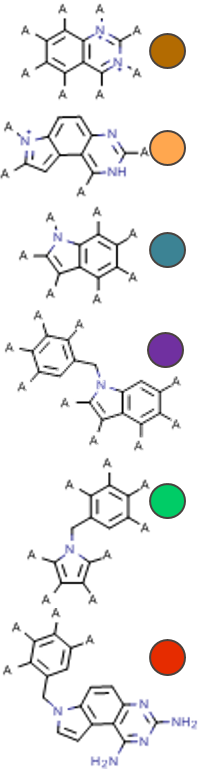
\includegraphics[width=0.5in]{fig/tcam2_541564_6scaf_col.png}
  \caption{
    (a) Distribution of number of fragments, out of nearly 6000 total, found in each molecule in the TCAMS dataset. (b) Compound $C$, chosen here as Molecule 2 (TCAMS Compound ID 541564, PubChem CID: 44531725) from previous figures.
    (c) Compound $C$ has 6 fragments derived using the NCATS R-group tool, shown in legend at right. The scaffold pie plot shows the structure group of $C$, restricted here to only compounds that share two or more fragments with $C$. This ensures that all compounds sharing just a single heteroaromatic ring are not in the same group, as chemists expect, and also reduces the group size -- 80 related molecules for this particular compound $C$.}
    \label{fig:strucgroup}
\end{figure}


Comparing the Frameworks and NCATS R-Group Tool for the TCAMS dataset using the above mentioned statistical metrics, we show the aggregate statistics over the entire dataset in \fref{statcomparetable}.  

\begin{figure}
  \begin{minipage}[c]{\linewidth}
\vspace{0pt}
\centering
\scalebox{.8}{
(a)\begin{tabular}{|c|ccc|c|}
    \hline
    {\bf Column} & {\bf P10} & {\bf Median} & {\bf P90} & {\bf Avg} \\
    \hline    
    {\bf $C_A$} & 420.00 & 1849.00 & 3203.50 & 1845.54 \\
    {\bf $C_B$} & 83.50 & 888.00 & 2151.00 & 1047.93 \\
    {\bf $CP$} & 0.05 & 0.43 & 0.76 & 0.41 \\
    {\bf $PI_A$} & 0.76 & 0.96 & 1.00 & 0.91 \\
    {\bf $PI_B$} & 0.09 & 0.53 & 0.87 & 0.50 \\
    {\bf $PIU_A$} & 0.13 & 0.47 & 0.91 & 0.50 \\
    {\bf $PIU_B$} & 0.00 & 0.04 & 0.24 & 0.09 \\
    {\bf $Frag_A$} & 10.00 & 32.00 & 74.00 & 38.96 \\
    {\bf $Frag_B$} & 2.00 & 5.00 & 11.00 & 5.93 \\
    {\bf $FragEff_A$} & 15.60 & 52.12 & 140.23 & 69.72 \\
    {\bf $FragEff_B$} & 21.25 & 150.80 & 454.00 & 211.80 \\
    \hline
  \end{tabular}
 }
(b)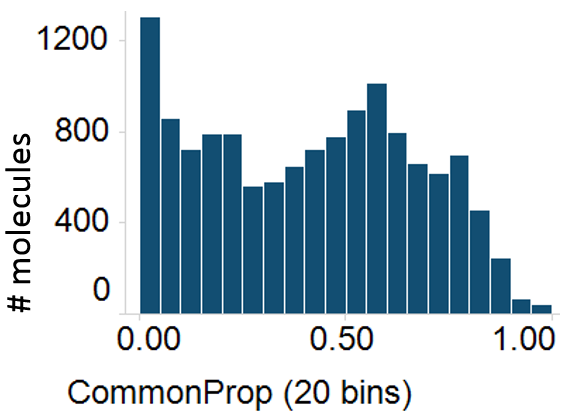
\includegraphics[width=2in]{fig/CP_TCAMS_GSKFW_RGT.png}
  \end{minipage}
  \caption{Statistics computed for 10th/90th percentile, median and average value for structure group size ($Ca$/$Cb$), common proportion, proportional information unique to A and B, number of fragments in and fragment efficiency of method A (frameworks) and B (NCATS R-group tool).}
\label{fig:statcomparetable}
\end{figure}


We compare the Common Proportion, Proportion of Information Unique (PIU) and Fragment Efficiency (FragEff) statistics for the Frameworks (method ``A'') and the NCATS R-group tool (method ``B'') for all the 13.5k compounds in TCAMS in \fref{statcompare}.  This figure has PIU of methods $A$ and $B$ on the axes, and is sized by the ratio of their Fragment Efficiencies for all 13.5k molecules.   



\begin{figure}
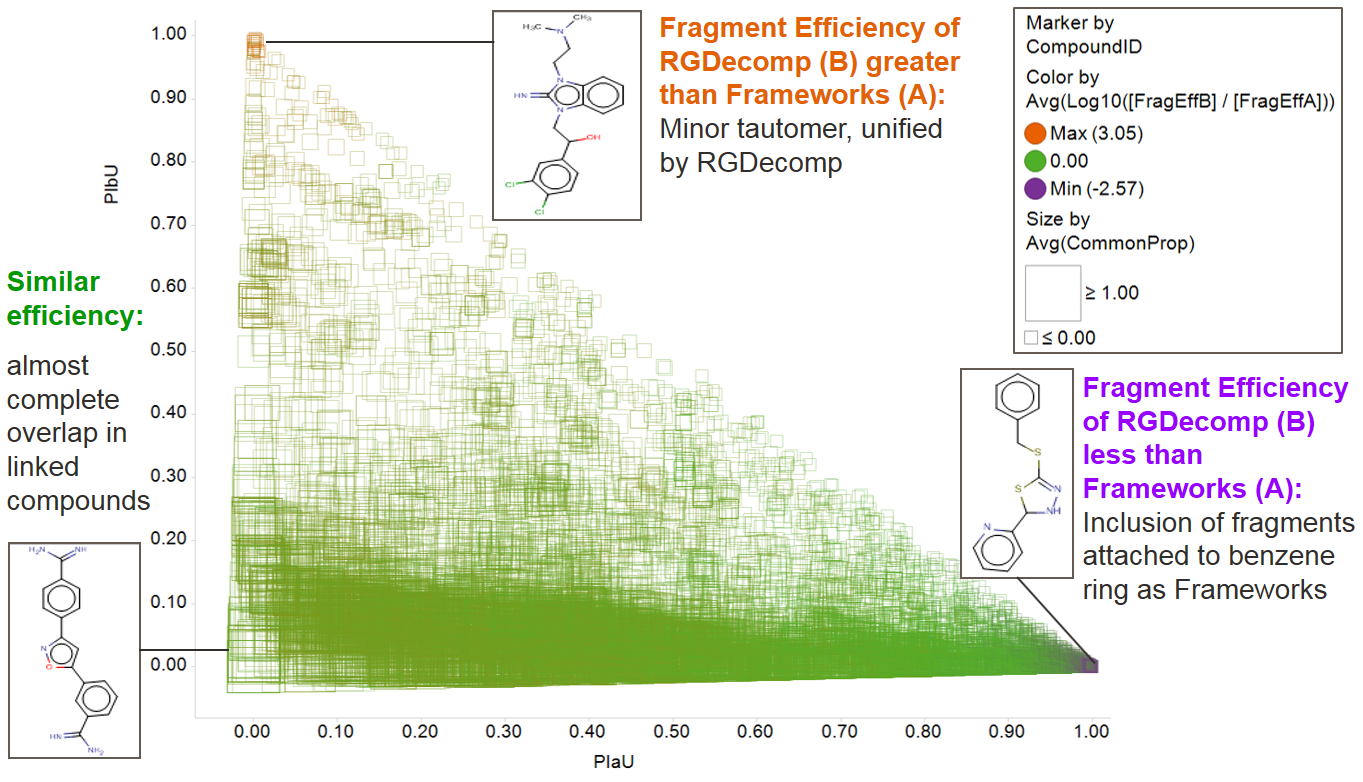
\includegraphics[width=6in]{fig/statcompare_frames_RGtool_transparent_density.png}
\caption{Comparison of the Common Proportion, PIU and FragEff statistics (described in the text) between Frameworks (method ``{\bf A}'') and NCATS R-group Tool (``{\bf B}'') for all molecules in TCAMS. PIU of A and B are on the X and Y axes, and the points are colored by the log ratio of FragEff(B) to FragEff(A) and sized by Common Proportion.}
\label{fig:statcompare}
\end{figure}
 
We can make a few observations from this data and plot:
\begin{enumerate} 
\item The two methods allow one to access different sets of molecules starting from any molecule in TCAMS - the average overlap in their coverage ($CP$) is 40\%, seen in Row 3 of \fref{statcomparetable}(a).  The distribution of $CP$ seen in  \fref{statcomparetable}(b) is bimodal with peaks at 0 and 55\%. The few molecules with almost complete overlap in coverage have high Common Proportion, low $PIU$ for both methods $A$ and $B$, and hence are represented by the large squares towards the bottom left of \fref{statcompare}. 
\item On the average, frameworks connected to a compound add more unique information than NCATS scaffolds connected to the same compound - this is seen in the higher density near the X-axis in \fref{statcompare}, and higher numbers for $PIU_A$ than $PIU_B$ in  \fref{statcomparetable}.   
\item On the average, one can link to about twice as many molecules with the frameworks, as seen by comparing $C_A$ to $C_B$ in \fref{statcomparetable}(a); however, this is because on the average there are 6 times more frameworks ($Frag_A$) than NCATS scaffolds ($Frag_B$). %, \ie NCATS scaffolds are three times more fragment-efficient for this dataset.  %, so the fragment efficiency is actually 3 times greater for NCATS scaffolds. %One could also argue that many of the framework-only links (\eg variously decorated benzene rings) are not useful.
\item The outliers are interesting. At one end, compounds in a rare tautomer are unified with the dominant one by the NCATS tool (high fragment efficiency), but left as singletons by the frameworks (low fragment efficiency). And compounds whose only link with other molecules would be a benzene ring or similar low complexity scaffold remain singletons with the R-group tool (lower fragment efficiency).
\end{enumerate}

\subsection{Statistical Basis of Structure-Activity Relationships (SAR)}\label{sec:statSAR}

We have also explored the Common Proportion measure to get at the overlap between structure and activity, \ie to investigate the statistical basis of SAR based on overlapping scaffolds. To do this, we define an Activity Group of compound $C$, $C_{act}$ as a set of compounds with activity bordering that of $C$ (in this case pIC50 in the 3D7 antimalarial assay). The activity group of each compound $C$ is defined to be the same size as the structure group, denoted $C_A$ or $C_B$ above, and generalized here as $C_{str}$.  This is done arbitrarily for ease of statistical calculations, being cognizant that it may sometimes lead to issues such as breaking a large list of compounds with the same activity arbitrarily, especially when picking a small list of activity neighbors for compounds with a small structure group.

The structure-activity common proportion, $CP_{str,act}(C)$ then measures the overlap between the structure neighbors of $C$, \ie compounds sharing any scaffold with $C$, and its activity neighbors, \ie compounds in a similar activity range.
\begin{equation}
CP_{str,act}(C) = \| C_{str} \cap C_{act} \| / \| C_{str} \cup C_{act} \|
\end{equation}

For comparing groups of different sizes we use the normalized Common Proportion, dividing by the expected overlap of the same activity group with a structure group determined purely by chance.  With the structure group being the same size as the activity group, this is the probability that if we pick $ \| C_{act} - 1\|$ compounds at random they will lie in $C_{act}$, \ie $(\| C_{act} - 1\|)/(N - 1)$. The subtraction by 1 accounts for the fact that the compound itself always lies in its own structure and activity neighborhoods. So then:

\begin{equation}
NormCP_{str,act}(C) = CP_{str,act}(C) / (Expected CP for Random Str) 
\end{equation}

We computed this NormCP measure for all compounds, which fit a normal distribution centered at 1, implying that for all compounds considered as an aggregate, structural similarity does not imply activity similarity.  However, the top 200 most active compounds, which are activity outliers, are also outliers in this normal distribution of NormCP as shown in \fref{NormCP}(a).

\begin{figure}
  (a)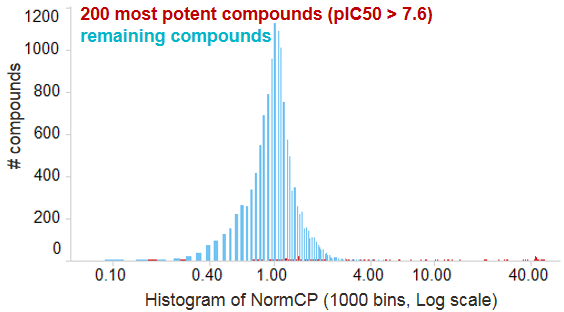
\includegraphics[width=4.5in]{fig/NormCP_all.png}\\
  (b)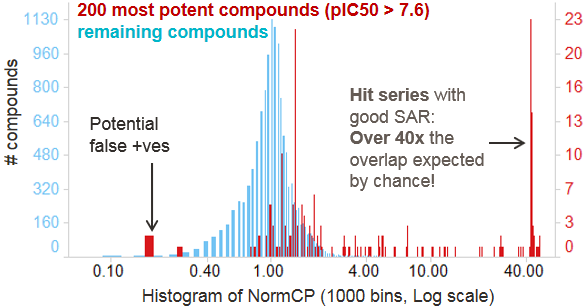
\includegraphics[width=4.5in]{fig/NormCP_top200.png}\\
  (c)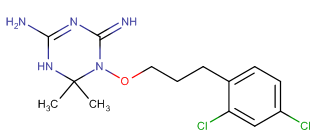
\includegraphics[width=1.5in]{fig/NormCP=42_5_pIC50=8_49_CID524739.png}
  (d)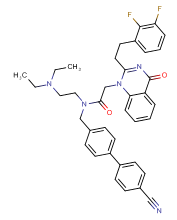
\includegraphics[width=1.5in]{fig/NormCP=0_17_pIC50=8_22_CID541941.png}
  (e)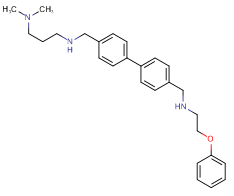
\includegraphics[width=1.7in]{fig/NormCP=0_16_pIC50=7_73_CID531249.png}  
  \caption{(a) Normalized common proportion scores between structure (data-driven frameworks) and activity ($pIC50_{3D7}$) for all 13.5k molecules in TCAMS.  The histogram has 1000 bins and a log scale on the X-axis. The top 200 most active compounds ($pIC50_{3D7}$ > 7.6) are marked in red, and occupy many of the outlier bars with high NormCP > 10. (b) Making the distribution of the top 200 active compounds clearer by giving them a separate scale, at the RHS. (c) One of the 23 compounds with NormCP = 42.5, Compound ID 524739. (d)--(e) two active compounds with low NormCP in the 0.16-0.17 range: (d) Compound ID 542941 and (e) Compound ID 531249. For both compounds, they alone are highly active among a structure group of 96 compounds, raising the probability that these compounds are flagpoles and not worth following up as hits.}
\label{fig:NormCP}   
\end{figure}

Among these compounds there are some that have over 40 times as much overlap between structure and activity than would be expected by chance, shown on the right of \fref{NormCP}(b) and in \fref{NormCP}(c).  This implies a strong confidence in the activity being genuine, and the series being worthy of making or measuring the activity of further analogs.

On the other hand, there are also some compounds, highlighted on the left side of \fref{NormCP}(b) and in \fref{NormCP}(d--e), that though they are among the top 200 by activity, have NormCP much less than 1, \ie much less overlap between structure and activity than would be expected by chance.  This would imply that structural neighbors of these compounds are largely less active that the original compound, no matter which of the overlapping scaffolds within the molecule we use to define those structural neighbors!  This gives us a way to quantify flagpoles or false positive hits, which may not be worth following up.

\section{Discussion}
\label{sec:discussion}

While threshold-based hit selection is a prevalent approach in the
analysis of high throughput screening datasets, it
ignores the extra information encoded in chemical structure. Thus,
scaffold based analysis of high throughput screening datasets
represents a truly data-driven approach to hit triage that attempts to
make use of \emph{all} the data collected from a high throughput
screen. Ranking scaffolds is a key step in prioritizing hits in a
scaffold-based approach, and while there are many ways to generate a
ranking, it is not obvious that there is a single, optimal method.

In this study we have presented some alternate approaches to scaffold
prioritization that make use of aggregate statistics based on
overlapping scaffolds, with the goal of providing a quantitative basis
for the comparison of different scaffold-based analysis schemes.
Also, the overlapping scaffold approach described here
avoids the phenomenon of similar molecules being arbitrarily assigned to
exclusive clusters, which affects partitioning-based methods such as
complete-linkage clustering as shown in \fref{clusterlanes}.
Instead, using overlapping scaffolds ensures that
molecules that differ only in decorations off a shared scaffold
will be considered within the same group.

Given the different ways to generate scaffolds and to compute
overlapping scaffolds, a quantitative approach to characterizing
differences in these approaches is necessary. The use of common
proportion ($\textrm{CP}$), fragment efficiency ($\textrm{FragEff}$)
and proportion of information unique to a method ($\textrm{PIU}$) 
places such differences within a sound statistical framework, allowing
for an objective comparison of fragmentation methods for a given
screen. They also extend the applicability of
methods to compare the output of different partitioning clustering
methods such as \citet{Torres2009}, allowing them to be used for
non-overlapping fuzzy clusters. Furthermore quantifying
structure-activity overlap using $\textrm{NormCP}$ is a novel
contribution, though similar in spirit and purpose to local hit rate
calculations that have been proposed for HTS triage\cite{Posner2009},
with a comprehensive structural neighbor metric based on overlapping
scaffolds.

We observe that the approach applied to triage the kinase ``X'' dataset
can be a powerful tool to identify promising hits.  The Spotfire workflow
is simple to implement and allows interactive drill-down from
aggregate properties to individual compounds. In essence,
the workflow described here enables decisions on individual compounds
using the aggregated data as a filter. Another advantage of this
workflow is that it supports the inclusion of ``virtual
datasets'' where there is no measured activity, as highlighted in the
data fusion use case.  Inclusion of such datasets can be useful as
they provide an opportunity to directly highlight untested regions of
chemical space. When multiple datasets are included in the data fusion, 
some with more accurately measured activities, it increases
confidence in noisy data by merging data for scaffolds across the
datasets.

In summary, the combination of anecdotal and statistical methods to
compare scaffold schemes and the resultant analysis of HTS datasets
highlights the fact that no single fuzzy clustering method is optimal,
and the most appropriate approach should be selected based on the
types of analyses described here. Screening scientists have traditionally
used ``chemical intuition'' to select and examine scaffolds, which can 
lead to biased selections of scaffolds and subsequently of
leads. Our Scaffold-Based Analytics approach described in this study
combines data and intuitive visualizations to help scientists combat such biases. 


\begin{acknowledgement}
  The GSK authors thank Subhas Chakravorty, Neysa Nevins, Ami Lakdawala Shah,
  Eric Manas, Todd Graybill, Stan Martens, Mike Ouellette, Tony Jurewicz, Rob
  Young, Ken Lind and Jeff Messer for valuable feedback and suggestions while developing the method and visualizations. We dedicate this work to the memory of Christopher Louer, our colleague and cheminformatics wizard at GSK who always encouraged us to innovate in order to help chemists.  
\end{acknowledgement}

%%%%%%%%%%%%%%%%%%%%%%%%%%%%%%%%%%%%%%%%%%%%%%%%%%%%%%%%%%%%%%%%%%%%%
%% The same is true for Supporting Information, which should use the
%% suppinfo environment.
%%%%%%%%%%%%%%%%%%%%%%%%%%%%%%%%%%%%%%%%%%%%%%%%%%%%%%%%%%%%%%%%%%%%%
\begin{suppinfo}
Supplementary material is available online for this article.
\end{suppinfo}

%%%%%%%%%%%%%%%%%%%%%%%%%%%%%%%%%%%%%%%%%%%%%%%%%%%%%%%%%%%%%%%%%%%%%
%% The appropriate \bibliography command should be placed here.
%% Notice that the class file automatically sets \bibliographystyle
%% and also names the section correctly.
%%%%%%%%%%%%%%%%%%%%%%%%%%%%%%%%%%%%%%%%%%%%%%%%%%%%%%%%%%%%%%%%%%%%%
%%\bibliographystyle{achemso}
\bibliography{bibliography}

\end{document}
